\definecolor{myGreen}{rgb}{0,0.6,0} %green

\begin{definition}[Triangles isométriques]
    Deux triangles sont \textbf{isométriques} lorsque leurs côtés sont deux à deux de même longueur.
\end{definition}

\begin{remarque}
    On peut également dire que les triangles sont \textbf{égaux}.
\end{remarque}

\begin{exemple*1}
    Les triangles $ABC$, $IJK$, $LMN$ et $XYZ$ se superposent par glissement et ou retournement, ils sont donc isométriques.
    \begin{center}
    \scalebox{0.6}{    
        \begin{tikzpicture}[line cap=round,line join=round,>=triangle 45,x=1cm,y=1cm]
            \clip(-9,-7) rectangle (9,5.5);
            \coordinate[label=below:$A$] (A) at (-7.74,1.07);
            \coordinate[label=below:$B$] (B) at (-1.28,2.07);
            \coordinate[label=above:$C$] (C) at (-4,4.51);
            \draw [line width=2pt,color=myGreen] (A)-- (B);
            \draw [line width=2pt,color=red] (B)-- (C);
            \draw [line width=2pt,color=blue] (C)-- (A);

            \coordinate[label=below:$I$] (I) at (0.7443407477719717,0.8432900996677757);
            \coordinate[label=above:$J$] (J) at (4.484340747771972,4.283290099667775);
            \coordinate[label=below:$K$] (K) at (7.204340747771972,1.8432900996677755);
            \draw [line width=2pt,color=myGreen] (I)-- (K);
            \draw [line width=2pt,color=red] (K)-- (J);
            \draw [line width=2pt,color=blue] (J)-- (I);

            \coordinate[label=above:$L$] (L) at (-8.642460471444396,-2.5698713621262446);
            \coordinate[label=above:$M$] (M) at (-2.1824604714443954,-1.569871362126245);
            \coordinate[label=below:$N$] (N) at (-5.922460471444396,-5.009871362126245);
            \draw [line width=2pt,color=myGreen] (M)-- (L);
            \draw [line width=2pt,color=red] (L)-- (N);
            \draw [line width=2pt,color=blue] (N)-- (M);
            
            \coordinate[label=above:$X$] (X) at (1.273312430294113,-1.521587110006146);
            \coordinate[label=above:$Y$] (Y) at (7.758729359192739,-2.340713021179218);
            \coordinate[label=below:$Z$] (Z) at (5.107961464351075,-4.855753690368624);
            \draw [line width=2pt,color=myGreen] (X)-- (Y);
            \draw [line width=2pt,color=red] (Y)-- (Z);
            \draw [line width=2pt,color=blue] (Z)-- (X);
        \end{tikzpicture}
    }
    \end{center}
\end{exemple*1}

% \pagebreak
\begin{propriete}[Premier cas d'égalité \admise]
    Si deux triangles ont un côté de même mesure compris entre deux angles de même mesure deux à deux alors ils sont \textbf{isométriques}.
\end{propriete}

\begin{exemple*1}
    \begin{itemize}
        \item \textcolor{red}{$AC$}=\textcolor{red}{$IK$}
        \item Le côté $[AC]$ est compris entre les angles \textcolor{blue}{$\widehat{CAB}$} et \textcolor{myGreen}{$\widehat{BCA}$}
        \item Le côté $[IK]$ est compris entre les angles \textcolor{blue}{$\widehat{IKJ}$} et \textcolor{myGreen}{$\widehat{JIK}$}
        \item \textcolor{blue}{$\widehat{CAB}$}=\textcolor{blue}{$\widehat{IKJ}$} et \textcolor{myGreen}{$\widehat{BCA}$}=\textcolor{myGreen}{$\widehat{JIK}$}
    \end{itemize}
    Donc les triangles $ABC$ et $IJK$ sont isométriques.
    \begin{center}
        \scalebox{0.6}{            
            \begin{tikzpicture}[line cap=round,line join=round,>=triangle 45,x=1cm,y=1cm]
                \clip(-11,-4) rectangle (5,2);
                \draw [shift={(-10,-2)},line width=2pt,color=blue,fill=blue,fill opacity=0.5] (0,0) -- (-9.462322208025617:0.6) arc (-9.462322208025617:56.309932474020215:0.6) -- cycle;
                \draw [shift={(-4,-3)},line width=2pt,color=myGreen,fill=myGreen,fill opacity=0.5] (0,0) -- (135:0.6) arc (135:170.53767779197437:0.6) -- cycle;
                \draw [shift={(-2,1)},line width=2pt,color=myGreen,fill=myGreen,fill opacity=0.5] (0,0) -- (-45:0.6) arc (-45:-9.462322208025615:0.6) -- cycle;
                \draw [shift={(4,0)},line width=2pt,color=blue,fill=blue,fill opacity=0.5] (0,0) -- (170.53767779197437:0.6) arc (170.53767779197437:236.3099324740202:0.6) -- cycle;
                
                \coordinate[label=below:$A$] (A) at (-10,-2);
                \coordinate[label=above:$B$] (B) at (-8,1);
                \coordinate[label=below:$C$] (C) at (-4,-3);
                \coordinate[label=above:$I$] (I) at (-2,1);
                \coordinate[label=below:$J$] (J) at (2,-3);
                \coordinate[label=above:$K$] (K) at (4,0);

                \draw [line width=2pt] (A)-- (B);
                \draw [line width=2pt] (B)-- (C);
                \draw [line width=2pt,color=red] (C)-- (A);
                \draw [line width=2pt,color=red] (I)-- (K);
                \draw [line width=2pt] (K)-- (J);
                \draw [line width=2pt] (J)-- (I);
            \end{tikzpicture}
        }
    \end{center}
\end{exemple*1}

\begin{propriete}[Deuxième cas d'égalité \admise]
    Si deux triangles ont un angle de même mesure compris entre deux côtés de même mesure deux à deux alors ils sont \textbf{isométriques}.
\end{propriete}

\begin{exemple*1}
    \begin{itemize}
        \item \textcolor{red}{$AC$}=\textcolor{red}{$IK$}
        \item \textcolor{myGreen}{$AB$}=\textcolor{myGreen}{$JK$}
        \item L'angle \textcolor{blue}{$\widehat{CAB}$} est compris entre les côtés \textcolor{red}{$[AC]$} et \textcolor{myGreen}{$[AB]$}
        \item L'angle \textcolor{blue}{$\widehat{IKJ}$} est compris entre les côtés \textcolor{red}{$[IK]$} et \textcolor{myGreen}{$[KJ]$}
        \item \textcolor{red}{$AC$}=\textcolor{red}{$IK$} et \textcolor{myGreen}{$AB$}=\textcolor{myGreen}{$JK$}
    \end{itemize}
    Donc les triangles $ABC$ et $IJK$ sont isométriques.
    \begin{center}
        \scalebox{0.6}{            
            \begin{tikzpicture}[line cap=round,line join=round,>=triangle 45,x=1cm,y=1cm]
                \clip(-11,-4) rectangle (5,2);
                \draw [shift={(-10,-2)},line width=2pt,color=blue,fill=blue,fill opacity=0.5] (0,0) -- (-9.462322208025617:0.6) arc (-9.462322208025617:56.309932474020215:0.6) -- cycle;
                \draw [shift={(4,0)},line width=2pt,color=blue,fill=blue,fill opacity=0.5] (0,0) -- (170.53767779197437:0.6) arc (170.53767779197437:236.3099324740202:0.6) -- cycle;
                \coordinate[label=below:$A$] (A) at (-10,-2);
                \coordinate[label=above:$B$] (B) at (-8,1);
                \coordinate[label=below:$C$] (C) at (-4,-3);
                \coordinate[label=above:$I$] (I) at (-2,1);
                \coordinate[label=below:$J$] (J) at (2,-3);
                \coordinate[label=above:$K$] (K) at (4,0);

                \draw [line width=2pt,color=myGreen] (A)-- (B);
                \draw [line width=2pt] (B)-- (C);
                \draw [line width=2pt,color=red] (C)-- (A);
                \draw [line width=2pt,color=red] (I)-- (K);
                \draw [line width=2pt,color=myGreen] (K)-- (J);
                \draw [line width=2pt] (J)-- (I);
            \end{tikzpicture}
        }
    \end{center}
\end{exemple*1}

\begin{propriete}[Triangles isométriques et conséquences \admise]
    Si deux triangles sont isométriques alors :
    \begin{itemize}
        \item leurs angles sont de même mesure;
        \item leurs aires sont égales.
    \end{itemize}
\end{propriete}

\begin{remarques}
    \emoji{warning} \emoji{warning} \emoji{warning}
    
    La réciproque n'est pas forcément vraie.
    \begin{itemize}
        \item Deux triangles peuvent avoir des angles deux à deux de même mesure, sans pour autant être isométriques. Nous verrons ça avec le théorème de Thalès.
        \item Deux triangles peuvent avoir la même aire sans être isométriques.\par
        \textbf{Contre-exemple ci-dessous} :  les triangles $ABC$ et $DEF$ ont une aire de 12 unités d'aire mais ne sont pas isométriques.
    \end{itemize}
    \begin{center}
        \scalebox{0.7}{
            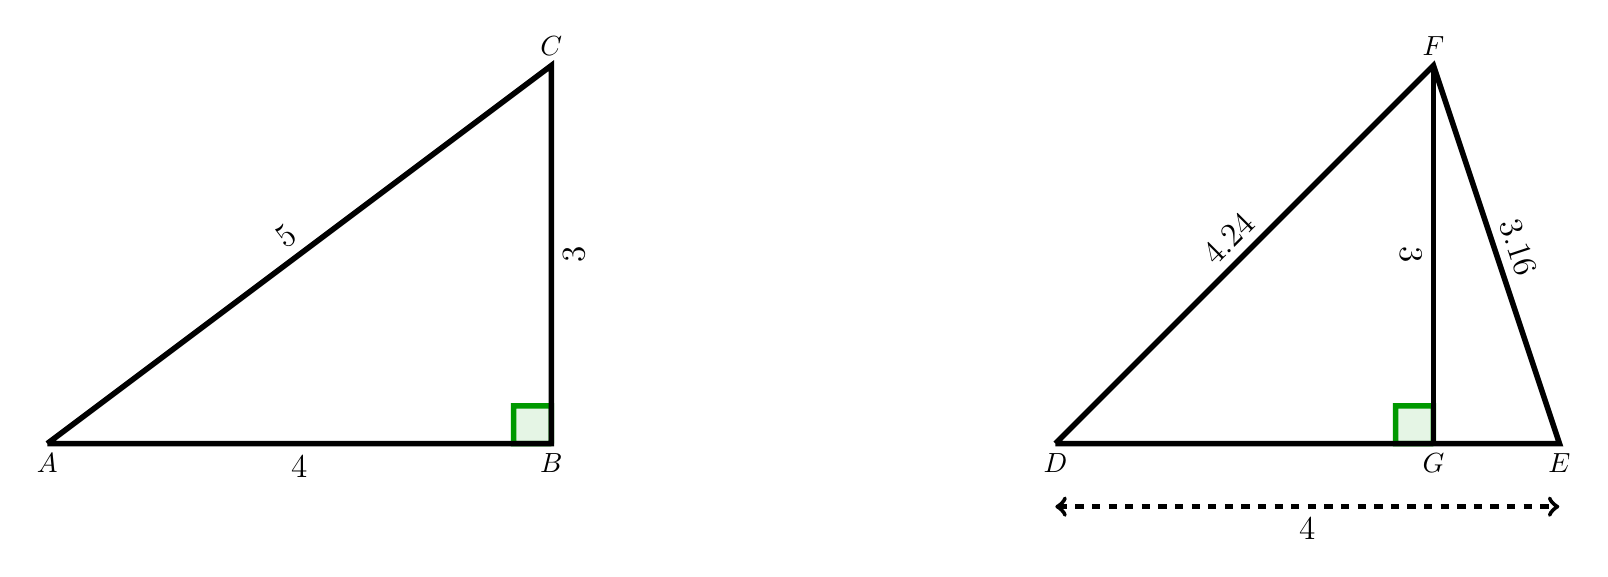
\begin{tikzpicture}[scale=1.6]                
                % \draw[help lines, color=black!30, dashed] (-8,0) grid (6,5);
                \coordinate[label=below:$A$] (A) at (-7,1);
                \coordinate[label=below:$B$] (B) at (-3,1);
                \coordinate[label=above:$C$] (C) at (-3,4);
                \coordinate[label=below:$D$] (D) at (1,1);
                \coordinate[label=below:$E$] (E) at (5,1);
                \coordinate[label=above:$F$] (F) at (4,4);
                \coordinate[label=below:$G$] (G) at (4,1);
                
                \draw[line width=2pt,color=myGreen,fill=myGreen,fill opacity=0.1] (B)--(-3.3,1)--(-3.3,1.3)--(-3,1.3)--(B);
                \draw[line width=2pt,color=myGreen,fill=myGreen,fill opacity=0.1] (G)--(3.7,1)--(3.7,1.3)--(4,1.3)--(G);

                \draw [line width=2pt] (A) -- node[sloped,below] {\large\Lg{4}} (B) -- node[sloped,below] {\large\Lg{3}} (C) -- node[sloped,above] {\large\Lg{5}} (A);
                \draw [line width=2pt] (D) -- (E) -- node[sloped,above] {\large\Lg{3.16}} (F) -- node[sloped,above] {\large\Lg{4.24}} (D);                
                \draw [line width=2pt] (F) -- node[sloped,below] {\large\Lg{3}} (G);

                \draw[<->,dashed, ultra thick] (1,0.5) -- node[sloped,below] {\large\Lg{4}} (5,0.5);
            \end{tikzpicture}
        }
    \end{center}

\end{remarques}
